% This is samplepaper.tex, a sample chapter demonstrating the
% LLNCS macro package for Springer Computer Science proceedings;
% Version 2.20 of 2017/10/04
%
\documentclass[runningheads]{llncs}
%
\usepackage{graphicx}
\usepackage{listings}
\usepackage{wrapfig}
% Used for displaying a sample figure. If possible, figure files should
% be included in EPS format.
%
% If you use the hyperref package, please uncomment the following line
% to display URLs in blue roman font according to Springer's eBook style:
% \renewcommand\UrlFont{\color{blue}\rmfamily}

\begin{document}
%
\title{Marlowe: implementing and analysing financial contracts\thanks{Supported by IOHK.}}
%
%\titlerunning{Abbreviated paper title}
% If the paper title is too long for the running head, you can set
% an abbreviated paper title here
%
\author{
Pablo Lamela Seijas\inst{1} \and
Alex Nemish\inst{1} \and
David Smith\inst{1} \and
Simon Thompson\inst{1,2}\orcidID{0000-0002-2350-301X}}
%
\authorrunning{P. L. Seijas, A. Nemish, et al.}

% First names are abbreviated in the running head.
% If there are more than two authors, 'et al.' is used.
%
\institute{IOHK, Hong Kong, \url{https://iohk.io} \\
\email{\{alexander.nemish, pablo.lamela, david.smith, simon.thompson\}@iohk.io} \and
School of Computing, University of Kent, UK\\
\email{s.j.thompson@kent.ac.uk}}
%
\maketitle              % typeset the header of the contribution
%



\begin{abstract}
The abstract should briefly summarize the contents of the paper in
150--250 words.

\keywords{First keyword  \and Second keyword \and Another keyword.}
\end{abstract}
%
%
%


\section{Introduction}

Intro
\section{Marlowe overview SJT}

Introduce the main types and informal overview of execution. Contrast with Marlowe 1.3 (as in ISoLA paper). Embedding in Haskell? [All this stuff is in the tutorial already]

\section{Implementation of Marlowe on the mockchain AN}

 [An updated version of the description in the Plutus platform paper]

\section{Analysing Marlowe contracts PLS}

Covers static analysis and Isabelle proofs [New]

\clearpage
\section{The Marlowe Playground}

For Marlowe to be usable in practice, users need to be able to understand how contracts will behave once deployed to the blockchain before actually deploying the contract. We can do that by simulating their behavior with a mockchain and interactively stepping through the evaluation of a contract in a browser.

To achieve this, and to aid Marlowe’s take-up usage by people who are not familiar with its syntax, we have developed the Marlowe Playground, a web tool that supports the interactive construction, revision, and simulation of smart-contracts written in Marlowe. The tool is publicly available in the url: https://prod.meadow.marlowe.iohkdev.io/. It should be mentioned that development of the playground is rapid and the latest unstable version is also publicly available at https://alpha.marlowe.iohkdev.io/.

The playground has an editor where you can write a contract in "pure" Marlowe, that is, not embedded in a host language. The reason for doing this is two-fold:
\begin{itemize}
    \item There is a shallower learning curve for users who are new to Haskell or programming languages in general. The Marlowe constructs are quite simple so there is no need to learn about Haskell syntax or even variables, functions etc.
    \item As we step through the execution of a contract, the contract is reduced, it is very useful to be able to view and even edit the reduced contract during this execution.
\end{itemize}
This is probably not the best way to write a large contract so the playground contains an additional editor where contracts can be written using Haskell and then transferred as a pure Marlowe data structure into the Marlowe editor.

In addition to pure Marlowe and Haskell editors, contracts can also be written using Google's Blockly visual programming language. Again this is not suitable for writing large contracts however it is an easy way to introduce the concepts of Marlowe to users who have no programming knowledge. Once a contract has been 'written' in Blockly it is possible to transfer that contract to the Marlowe editor. It is also possible to transfer a Marlowe contract to Blockly for further editing.

The Marlowe editor in the unstable version of the playground has an additional feature to aid writing contracts called holes. If we enter the contract \lstinline{?mycontract} we will be presented with a dropdown list of values that could be used.

\begin{wrapfigure}[5]{l}{0.25\textwidth}
    \vspace*{-0.3in}
    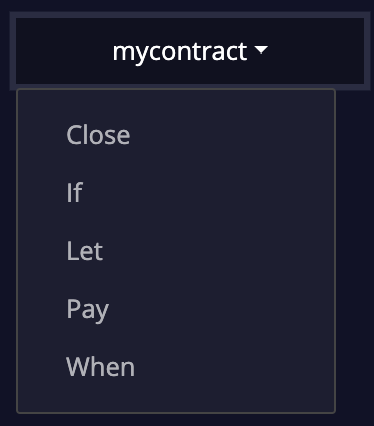
\includegraphics[width=0.25\textwidth]{hole_options.png}
\end{wrapfigure}
In our case \lstinline{?mycontract} must be a \lstinline{Contract} of some sort so we can choose one of the \lstinline{Contract} constructors from the dropdown list. If we choose \lstinline{Pay} then the Marlowe editor will automatically fill in a skeleton \lstinline{Pay} contract with new holes where we need to provide values.
\\ \\
\begin{verbatim}
    Pay ?accountId_1_1 ?payee_1_2 ?value_1_3 ?contract_1_4
\end{verbatim}
New options will be presented, one for each hole, and each will have a dropdown list of all the possible values.
\begin{wrapfigure}[6]{l}{0.25\textwidth}
    \vspace*{-0.3in}
    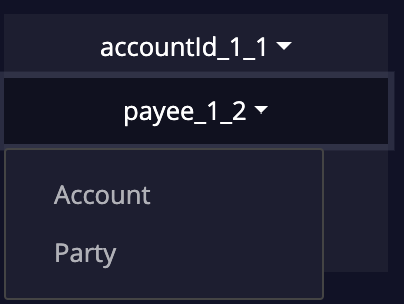
\includegraphics[scale=0.2]{hole_options_2.png}
\end{wrapfigure}
A complete contract can be written in this guided way with the user needing only to fill in strings and numbers by hand. This approach to writing holes in your code and "asking" the compiler what you could put in there is easy to implement in a DSL as there are very limited options however is is becoming popular with more complex languages such as Haskell and Idris.

Contracts written in the Marlowe editor are parsed in real-time and if there are no errors (and no holes) then the contract is analyzed to discover which actions a user could take to progress the contract. These actions are displayed in the "Input Composer" above the editor. Lets take the following example contract:
\begin{verbatim}
    When [Case (Deposit (AccountId 0 "investor") "guarantor" (Constant 1000)) 
    Close] 10 Close
\end{verbatim}
In this case, the only action a user can take to progress the contract is to deposit 1000 ADA from the guarantor to the investor's account. The playground knows this and so the input composer displays this action in the input composer.

\begin{figure}[]
    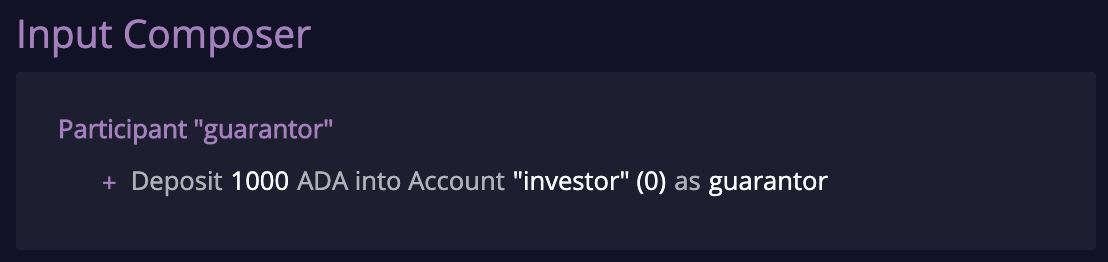
\includegraphics[width=1\textwidth]{input_composer.png}
\end{figure}
The user can then choose to add this action to a transaction, ready to be applied. Multiple actions can be added to a transaction before it is applied if such actions are meaningful.

\begin{figure}[]
    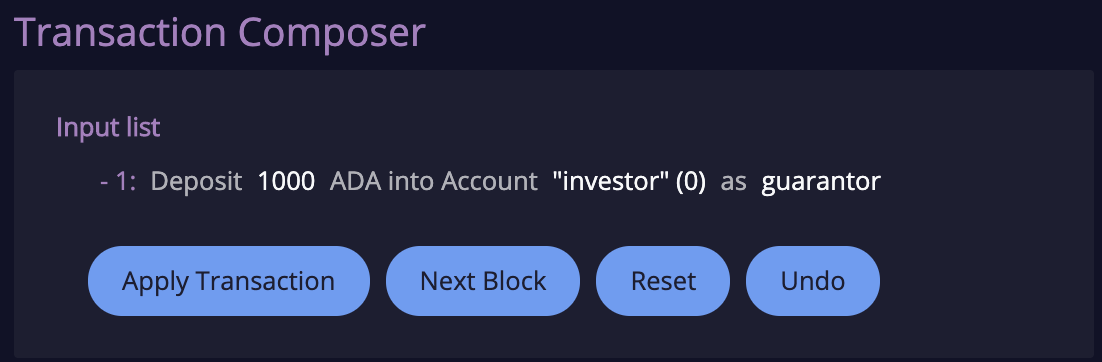
\includegraphics[width=0.8\textwidth]{tx_composer.png}
\end{figure}
A user can then apply this transaction and in the example above this would result in the state pane showing a single payment and in addition the Contract in the Marlowe editor will have been reduced to \lstinline{Close}. At this point a user can undo the application of the transaction or even reset the contract to it's initial state. This enables a user to apply transactions, see what the effect is, step back and apply a transaction with different actions and see how these differences effect the end results. They can also change the reduced contract to investigate a different path.

Users can at any point save their contract directly to a Github Gist and of course load a contract from a Github Gist. There are also some demo contracts that can be loaded in order to play around with realistic examples.

The final feature that we would like to present is the static analysis of contracts. As mentioned in a previous section, it is possible to carry out a symbolic execution of a contract and then use a SMT solver to look for cases that could cause unwanted situations. The playground utilizes this to search for situations where contract execution would cause warnings. For example, suppose you write a contract that causes a payment of 450 Lovelace from Alice to Bob but the contract allows a situation where Alice has only deposited 350 Lovelace then the static analysis will find this and report it to the playground user.
\begin{figure}
    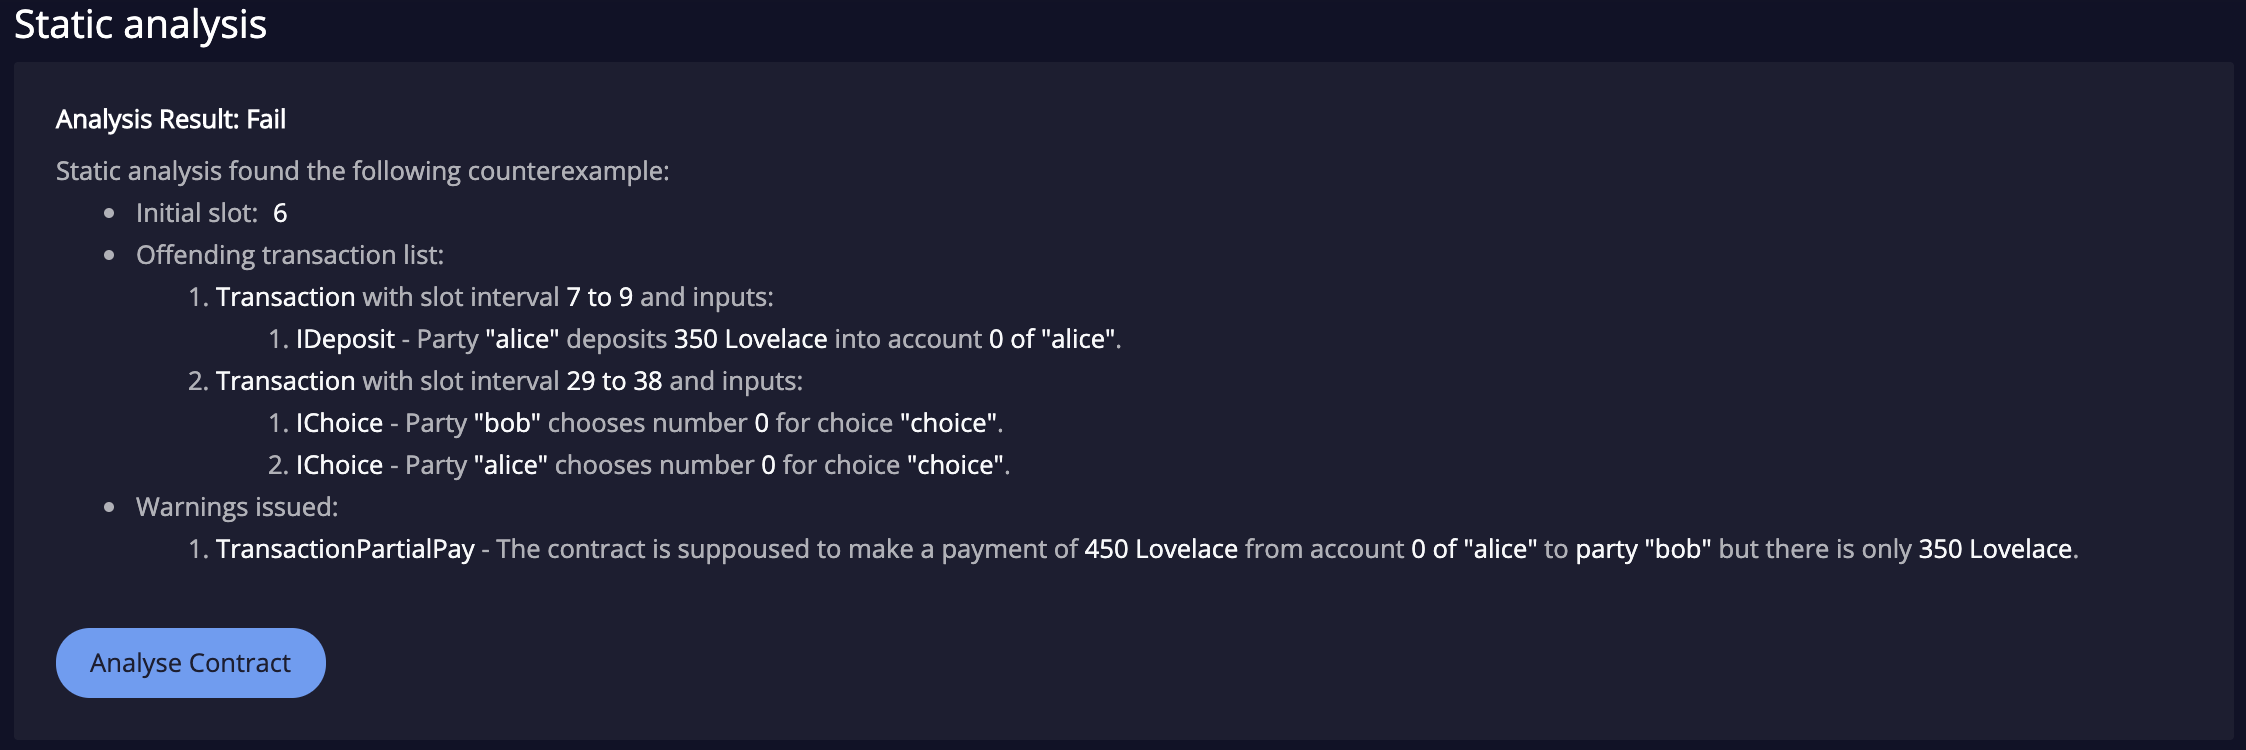
\includegraphics[width=1\textwidth]{static_analysis.png}
\end{figure}
\clearpage
\section{Related work}

Need to update from ISoLA paper \cite{isola-marlowe}.

\section{Future work and conclusions}

\section*{Left in for info \ldots}

\begin{figure}
% 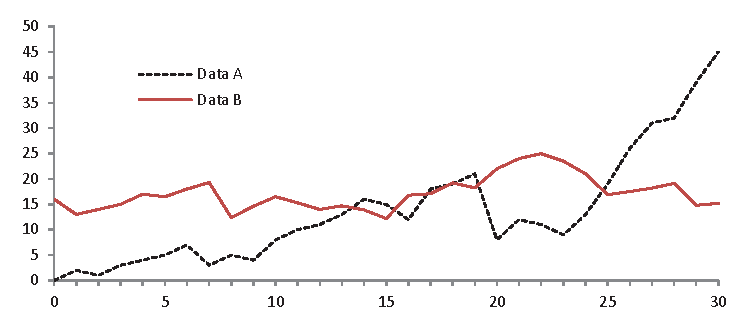
\includegraphics[width=\textwidth]{fig1.eps}
\caption{A figure caption is always placed below the illustration.
Please note that short captions are centered, while long ones are
justified by the macro package automatically.} \label{fig1}
\end{figure}


%
% ---- Bibliography ----
%
% BibTeX users should specify bibliography style 'splncs04'.
% References will then be sorted and formatted in the correct style.
%
\bibliographystyle{splncs04}
\bibliography{paper}
%
\end{document}
